%!TEX root = ../paper.tex

\subsection{Clustering}
\label{sec:clustering}

After extracting all features and vectorizing them for each blog post in the database, they are grouped together into clusters according to the similarity of their feature vectors.
To this end, we use a k-means algorithm which is a method from vector quantization.
Afterwards the resulting clusters are labeled, so that the user knows what kind of blog posts he can expect in a specific cluster.

\subsubsection{K-Means Algorithm}
\label{sec:k-means}
K-means creates $k$ clusters from $n$ vectors by randomly selecting $k$ points from the vector space as cluster centroids.
Then, each vector or point is assigned to its nearest cluster centroid according to its Euclidean distance to those centroids.
Afterwards, the cluster centroids are repositioned to the center of all vectors/points which were assigned to them.
These last two steps are repeated until the cluster centroids converge.
The resulting assignment of the vectors (and thus their corresponding blog posts) to the clusters is the same as the final assignment performed by the k-means algorithm.
For our implementation we used the k-means algorithm offered by Mahout\footnote{\url{https://mahout.apache.org/}}, which can be executed efficiently among a cluster with a large amount of data~\cite{esteves2011k}.

To run a k-means algorithm, the value $k$ has to be set beforehand.
$K$ represents the number of clusters and thus the number of similar writing styles, which should be determined.
Finding an appropriate value for $k$ depends highly on the use case.
One use case could be to find exact authors, so that one cluster, i.e. writing style group, would correspond to one author.
One cluster would only contain blog posts of one author.
The value $k$ should therefore be similar to the number of expected authors.
Another use case could be to find similar writing style groups.
One cluster would then contain blog posts from multiple authors having a similar writing style.
In this case $k$ should be chosen much lower than the actual number of authors.

% [TODO: Graphic?]
% [TODO: discuss other algorithms?]

\subsubsection{Cluster Labelling}
\label{sec:cluster_labeling}
Labelling the resulting clusters helps the user to distinguish between those.
The labels indicate what kind of blog posts are in those clusters, so that the user gets a feeling about what to expect from a blog posts of a specific cluster.

The current research in the field of cluster labelling focuses on topic-dependent labels.
Because we focus on the writing style rather as on the topic, we could not use those techniques.
Searching for universally accepted writing styles leads to labels like ``informative'' or ``opinion piece'', which represents the text's intention [TODO: reference].
Also this standard could not be used in our approach.
[TODO: umschreiben!]

Therefore, we implemented our own cluster labelling methods, which consider the most important features of a cluster.
The methods are explained using the following example:
The current feature is ``length of blog posts'' and we have three clusters with the following values for the current feature:
\begin{center}
\begin{tabular}{c|c|c}
  Cluster 1 & Cluster 2 & Cluster 3 \\ \hline
  0.7 & 1 & 0.1 \\
 \end{tabular}
\end{center}
\paragraph{Method 1}
For each feature and cluster the highest and lowest value is determined.
Those cluster are then labelled with appropriate labels.
In the example cluster 2 has the highest value and gets the label ``longest blog posts''.
The label ``shortest blog posts'' is assigned to cluster 3, because this cluster has the lowest value.
Using this method only the most significant labels are set.
But, it can happen that a cluster does not obtain any label.

\paragraph{Method 2}
First the average vector of all blog posts is calculated.
Afterwards the distance for each feature and cluster to that average vector is determined.
If the distance is over a certain threshold, the cluster is labelled.
The example is shown in Figure~\ref{cluster_labeling_2}.
Because cluster 3 is not over the threshold, thus the length of the blog post is not significant for the cluster, no label is assigned to that cluster.
Cluster 1 and 2 are both over the threshold and obtain the label ``long blog posts''.
This method assigns more labels to clusters than method 1, but can also lead to clusters without any labels.

\begin{figure}[ht]
	\centering
	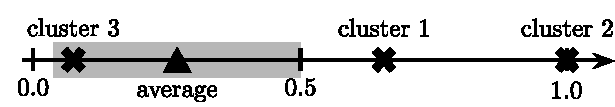
\includegraphics[width=0.33\textwidth]{images/cluster_labeling_2.pdf}
	\caption{}
	\label{cluster_labeling_2}
\end{figure}

\paragraph{Method 3}
As with Method 2, we calculate the difference to the average for each cluster and feature.
However, we also normalize them to the total range this feature has for our data.
Then, we pick the $n$ most significant of these differences for each cluster and use them to label it.
Significance, in this case, is mostly determined by how great the deviation from the average is: The larger the deviation the higher the significance.
The only exception to this is that being very close to to the average is considered slightly more significant than only being fairly close to it.
With this method, every cluster is guaranteed to get a set number of labels, even if it has no features that deviate from the average.
